\documentclass{article}
\usepackage{graphicx}
\usepackage{hyperref}
\usepackage[utf8]{inputenc}
\usepackage{lipsum}
\usepackage{courier} %% Sets font for listing as Courier.
\usepackage{listings, xcolor}
\usepackage{biblatex}

\addbibresource{test.bib}

\lstset{
tabsize = 4, %% set tab space width
showstringspaces = false, %% prevent space marking in strings, string is defined as the text that is generally printed directly to the console
numbers = left, %% display line numbers on the left
commentstyle = \color{green}, %% set comment color
keywordstyle = \color{blue}, %% set keyword color
stringstyle = \color{red}, %% set string color
rulecolor = \color{black}, %% set frame color to avoid being affected by text color
basicstyle = \ttfamily , %% set listing font and size
breaklines = true, %% enable line breaking
numberstyle = \tiny,
}

\title{Professional Practice in IT Project}
\author{
  Conor Shortt\\
  \href{https://github.com/conorshortt123}{Github}
  \and
  Blaine Burke\\
  \href{https://github.com/BurkeBlaine1999}{Github}
  \and
  Mark Reilly\\
  \href{https://github.com/MarkReillyGMIT}{Github}
}
\date{\today}

\begin{document}

\begin{figure}
    \centering
    
\includegraphics[scale=0.3]{./images/gmit.jpg}
\end{figure}

\maketitle


\tableofcontents
\newpage


\section{Introduction}
For our 3rd year project for professional practice in IT, we decided to design a full stack web application which uses Facial recognition software\cite{ageitgey} to log into a web page which
in turn allows the user to search a database to view other users information.\medskip

For the Front-end portion we chose to use Flask which is a micro framework written in Python,we chose Flask because it is extremely flexible, relatively easy to learn and use, and allows for more control over what components to use such as the type of database.\medskip

For the Back-end portion after a lot of research and testing for different ways to achieve communication between Front and Back end, the decision was made to use MongoDB.During the first few weeks we used Flask-SQLAlchemy but later changed to MongoDB which allowed the database to be accessed remotely by each project member.\medskip

Our main objectives for the project were:
\begin{enumerate}
\item Have a working login system using facial recognition
\item Improve communication skills in a project based environment 
\item Learning new technologies
\item Learning more about database communication
\end{enumerate}

\newpage

\section{System Requirements}
In order to run the project, there are several requirements needed.
\begin{itemize}
  \item A webcam is required to use the App as when it comes to logging in you will be prompted to scan your face for two factor authentications.  You are also required to upload a self-portrait Image of yourself in order to register an account.
  \item You are required to install the latest version of \href{https://www.python.org/downloads/}{python 3.}\cite{python}
  \item The project decencies are required to run our application. To install them follow the steps below! 
    \begin{enumerate}
    \item Clone the project to your desktop.
    \item Open the project and open command prompt
    \item Enter ‘pip install -r requirements.txt’ to download the dependencies
    \end{enumerate}
    \begin{center}
        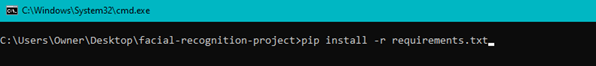
\includegraphics[scale=0.8]{images/requirementsInstall.png}
    \end{center}
  \item You are required to have \cite{cmake}\href{https://cmake.org/}{Cmake} and \cite{dlib}\href{http://dlib.net/}{Dlib} installed
  \item A text/Script editor you have installed. For example Visual Studio Code
\end{itemize}

\begin{center}

\includegraphics[scale=0.10]{./images/Python-logo.png}
\\

\includegraphics[scale=0.7]{images/cmake75.png}
\end{center}

\newpage

\section{Technology Used}
In the process of making our project we used several different technologies.
\begin{enumerate}
\item \href{https://www.python.org/downloads/}{Python} \\
We used python as our programming language as it has wide variety of libraries we could use making it our best option over other languages. Python is also very simple to use , proof being that this is our first python project .


\item \cite{flask}\href{https://flask.palletsprojects.com/en/1.1.x/}{Flask} \\
We used Flask as our python framework for our web application. 
Flask is a small and powerful web framework for Python. 
It's easy to learn and simple to use, enabling you to build your web app in a short amount of time. Flask can be used for building complex, database-driven websites
We chose flask due to its extensive documentation online so if we had issues we could easily find a solution to any problem.


\item \href{https://www.mongodb.com/}{MongoDB} \\
MongoDB is an open source database management system (DBMS) that uses a document-oriented database model which supports various forms of 
Data. This is one reason we chose it as we have several different types of data we needed to add such as numpy and binary arrays. It  also has  a very flexible data model and is very easy to learn!

\item Webcam \\	
We chose to use a webcam as we required one for facial recognition.
A webcam is essential for our application as without a webcam the user cannot login to our App due to our facial recognition two factor authentication. 
Any webcam should work that is connected to your Computer.

\item \cite{PIL}\href{https://pillow.readthedocs.io/en/stable/}{PIL} \\
PIL is the Python Imaging Library by Fredrik Lundh and Contributors.
We used PIL to convert images to bytes then to base 64 so we can easily store it on our database.

\item \href{https://github.com/ageitgey/face_recognition}{Face recognition Module} \\
We used  \href{https://github.com/ageitgey}{Adam Geitgeys} \href{https://github.com/ageitgey/face_recognition}{Face recognition Module} in our project for our two factor authentication when logging in.
\\
\\
\\
\\
\\
\end{enumerate}

\newpage

\section{Design Methodology}
When starting our project we specified our language we would use, our end goals  and what imports we could use.\medskip

\textbf{Setting our End Goals} \\
When we began our project, we, as a team decided on some end goals for our project.  We chose that our project would be a web application made using Python that uses facial recognition when logging in, in order to access a database containing all the user’s data.
At first, we were caught between the Flask and Django framework. Ultimately, we chose flask because it’s a small and powerful web framework, it’s easy to learn, flexible and simple to use.\medskip

\textbf{Choosing our storage method} \\
After deciding which framework we were going to use, we had to then chose which type of database was best to use with Flask. At the beginning we picked Flask-SQLAlchemy as it work very effectively and easily with Flask. After much consideration we decided that it would be best to change to using MongoDB because it would allow all the data in the database to be accessed remotely by each of us.\medskip

\textbf{Step One - Prepare the 3 main aspects individually} \\
After this we all began to work individually to get the three main aspects of the project functioning. These are the Facial recognition API , the backend server and the frontend built with flask. We spent approximatly 2 to 3 weeks building these individually. Once completed we began to implement them together.\medskip

\textbf{Step Two - Integration} \\
We began by taking the server and integrating it into the flask app. This was due to the fact that implementing the Facial recognition required the login and register to be working before it could be used.
Once the backend was implemented we added the facial recognition API as our two factor authentication.\medskip

\textbf{Step Three - Improving efficiency} \\
With the whole app finally together we set out on improving the apps overall efficiency by  removing any unnecessary code that was left in. During this process we greatly improved the time it takes to launch the localhost server.\medskip

\textbf{Step Four - Improve accesibility,Ergonomics and clean up} \\
Now that the bulk of the work was done we had to clean up our code and UI. We began to add more detailed,updated comments to our code to make it more accessible to others. We made our Flask app more ergonomic so anyone using the app for the first time could easily understand how it works! During this process we also improved the overall aesthetics of the Application.

\begin{figure}[h!]
\centering
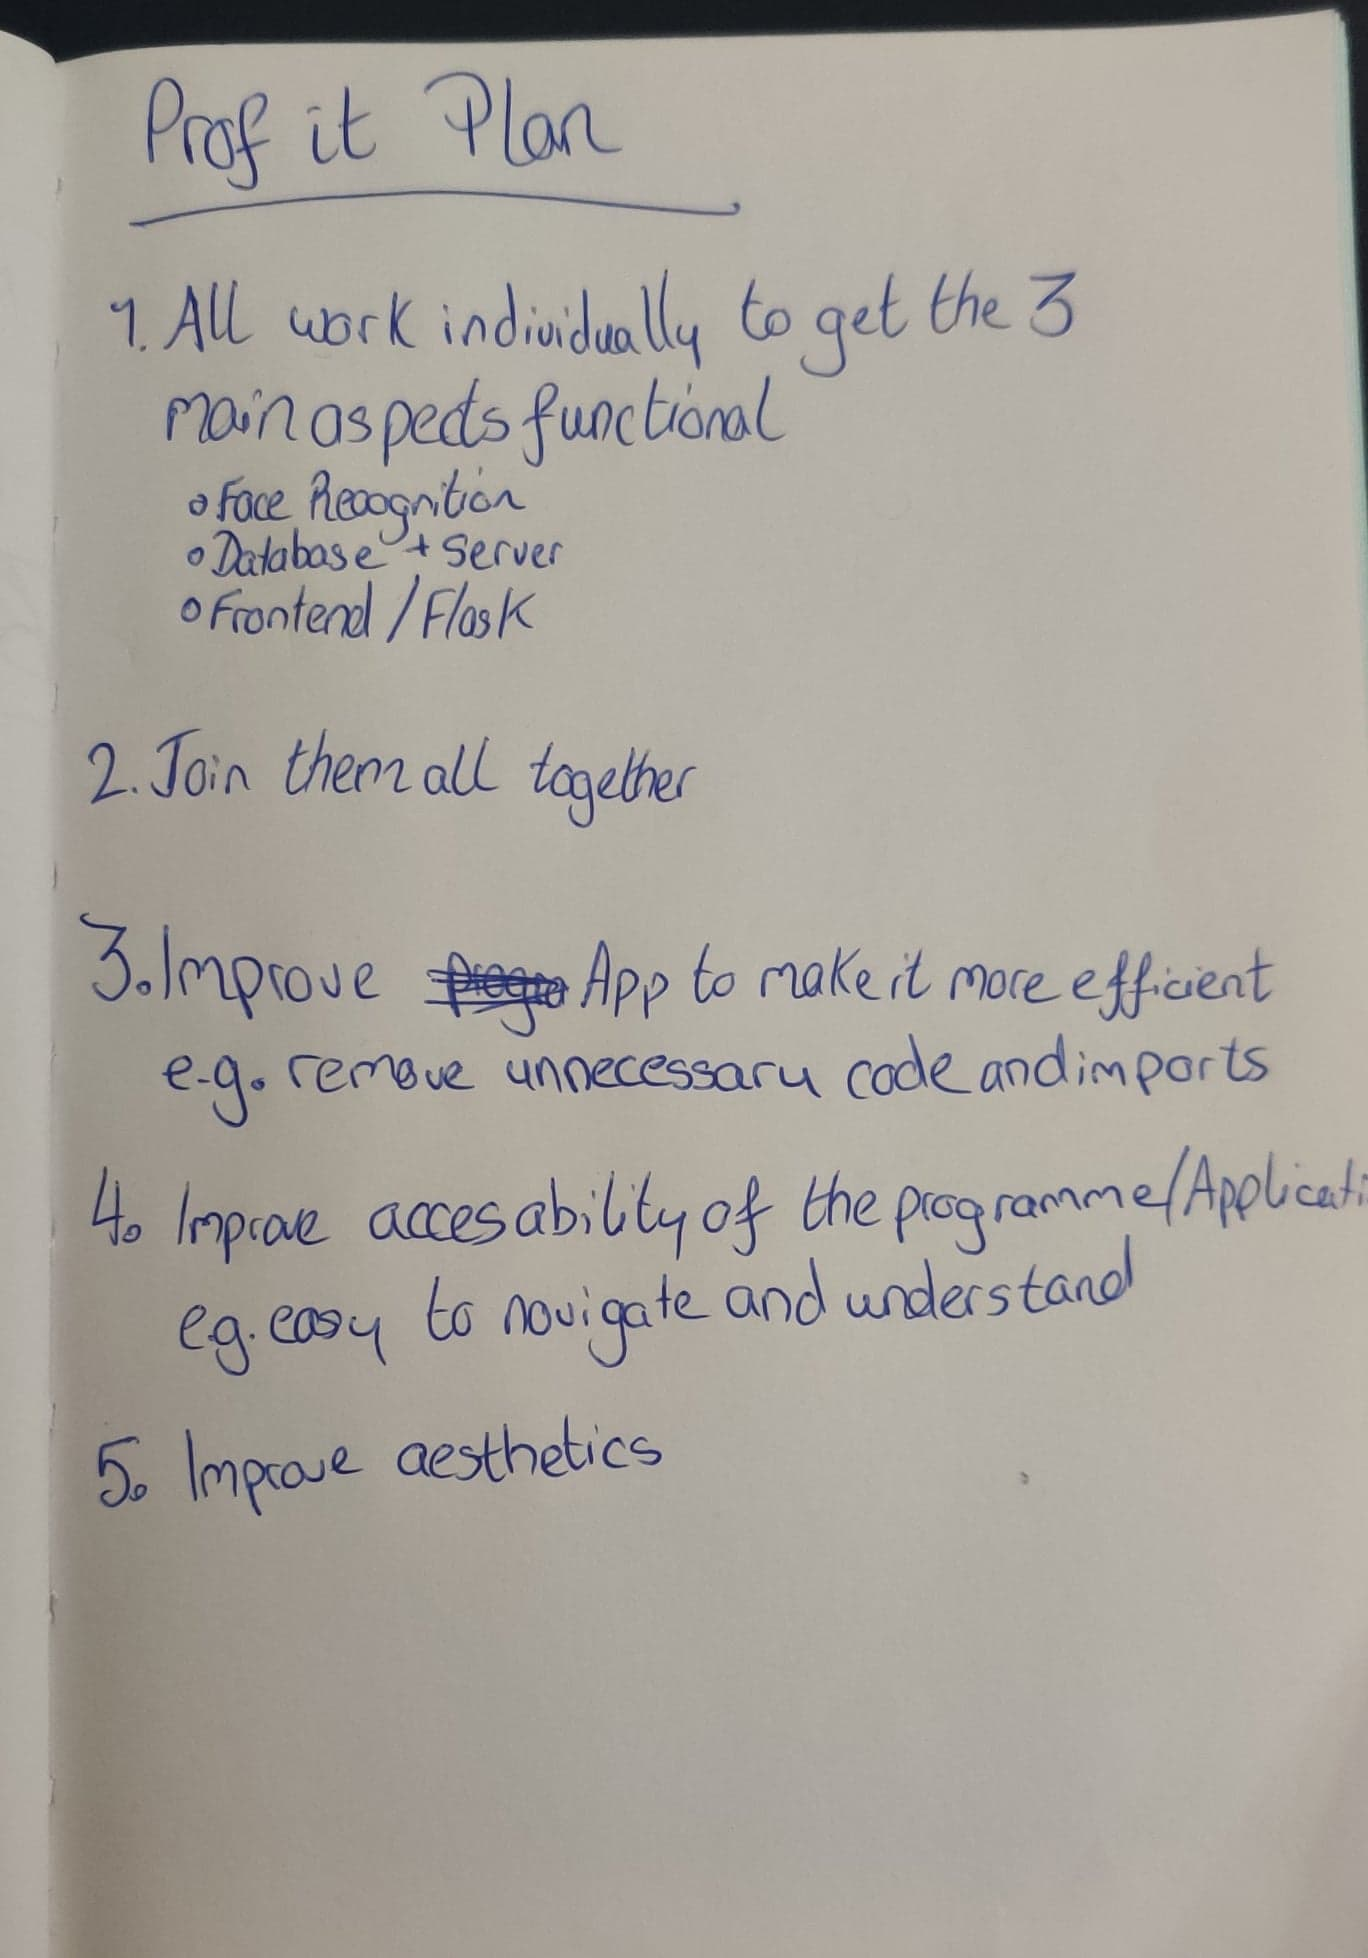
\includegraphics[scale=0.14]{images/Plan.jpg}
\caption{Our initial plan }
\end{figure}
\newpage

\section{Limitations and known bugs}
Throughout the course of making out project we encountered many bug and limitations but we gradually over came them and worked around them.
\begin{enumerate}
\item MongoDB \\
When it came to connecting the MongoDB server, at first it would not connect and would throw errors whenever we tried to call from it. After several YouTube tutorials and after scrolling through several different stack overflow forums we figured it out and implemented the fixes. 
\item Dlib \\
With Dlib we found it tough to get it installed correctly. In the beginning we could not figure out to get it installed properly as it would keep throwing errors every time, we called it. In the end with some research and determination we eventually got Dlib correctly working on our systems
\\
\\
\\
\\
\\
\\
\\
\\

\end{enumerate}

\newpage

\section{Features of the Implementation}

There are several features available in our project.
\begin{enumerate}
    \item A Register system that requires several details such as the username and stores the details to a database.
    Due to our databases primary key being the username, they must all be different.
    \item A Login system that validates the Users Username and password by checking if they match the records in the database, once their credentials are verified they are brought to a facial 
    \item A Login / Logout system that allows the current user of a session to logout once logged in to allow another user to log in on the same device!
    \item A search bar that allows the user to search through the database  via username and retrieve the users profile.
    This contains their profile photo , username and email.
    \item An account button that allows the current user to view their own profile.

\end{enumerate}

\newpage

\section{Testing Plans}

When it came to testing out our App we used mostly white box testing where the tester knows the internals of the code being tested and a small bit of black box testing where the tester knows nothing of the internals of the code.
\\
\\
White box testing allowed us to test our code faster and more efficiently but black box testing proved useful as it gave us the opinion of an outside source  , helping us get more ideas and opinions and allowed us to see if our app is ergonomic to a wide range of users and easy to navigate through.

\newpage

\section{Recommendations for Future Development}
There are many aspects of this project that could be expanded upon after the duration of the allotted project time. We were limited by time but certainly we could improve many aspects of our software. There were three main areas that we developed as part of our project. I developed the facial recognition scripts and camera, Blaine developed the \cite{mongodb}MongoDB backend aspect, and Mark developed the frontend Flask web
application.
\\
\subsection{Current State of the Software}
Currently the software is extremely malleable and not concrete by any means. It could certainly be taken in almost any direction. As of right now it features a database connected to the frontend flask application. With two factor authentication (Enter details and also facial recognition) as part of logging in. This software could potentially be used in several ways as I will highlight below.

\subsection{Potential Future Uses}
\textbf{Student Database}\\\\
We discussed many ideas and plans of what we were going to aim for when making the software, we settled on a database where we could search for a student username and it would get their details from the database and return them. The idea is that this is tailored towards teachers where they log in with two factored authentication using their details and their face.
\\\\\\
\textbf{Criminal Records Database}\\\\
Another direction that this software could easily be brought in is a criminal records database. The user of this software would be a police officer or a prison warden perhaps. They log in with their details and face and then can subsequently scan a persons face who they have possibly stopped on the road, if the persons face is registered in the database it will pull down their details.
\\\\\\
\textbf{Database for Employees}\\\\
The database could also be geared for industrial use. If an employer needed to keep track of where every employee was in the company site for example they could set up a camera system, connected to a computer which took frames from the cameras and compared faces in each camera to the database of employees, if someone not registered as an employee entered the building, an alert of some sort could be triggered.
\\\textbf{Home Security}\\\\
The database could be set up for a household where every person in the house is registered in the database. A camera is mounted at the entrance to the home and whenever someone is detected in the camera a computer connected to the camera performs facial recognition and lets them in depending if their face is registered in the database or not.

\newpage

\section{Conclusions}


\newpage
\printbibliography

\end{document}
